\documentclass[1p]{elsarticle_modified}
%\bibliographystyle{elsarticle-num}

%\usepackage[colorlinks]{hyperref}
%\usepackage{abbrmath_seonhwa} %\Abb, \Ascr, \Acal ,\Abf, \Afrak
\usepackage{amsfonts}
\usepackage{amssymb}
\usepackage{amsmath}
\usepackage{amsthm}
\usepackage{scalefnt}
\usepackage{amsbsy}
\usepackage{kotex}
\usepackage{caption}
\usepackage{subfig}
\usepackage{color}
\usepackage{graphicx}
\usepackage{xcolor} %% white, black, red, green, blue, cyan, magenta, yellow
\usepackage{float}
\usepackage{setspace}
\usepackage{hyperref}

\usepackage{tikz}
\usetikzlibrary{arrows}

\usepackage{multirow}
\usepackage{array} % fixed length table
\usepackage{hhline}

%%%%%%%%%%%%%%%%%%%%%
\makeatletter
\renewcommand*\env@matrix[1][\arraystretch]{%
	\edef\arraystretch{#1}%
	\hskip -\arraycolsep
	\let\@ifnextchar\new@ifnextchar
	\array{*\c@MaxMatrixCols c}}
\makeatother %https://tex.stackexchange.com/questions/14071/how-can-i-increase-the-line-spacing-in-a-matrix
%%%%%%%%%%%%%%%

\usepackage[normalem]{ulem}

\newcommand{\msout}[1]{\ifmmode\text{\sout{\ensuremath{#1}}}\else\sout{#1}\fi}
%SOURCE: \msout is \stkout macro in https://tex.stackexchange.com/questions/20609/strikeout-in-math-mode

\newcommand{\cancel}[1]{
	\ifmmode
	{\color{red}\msout{#1}}
	\else
	{\color{red}\sout{#1}}
	\fi
}

\newcommand{\add}[1]{
	{\color{blue}\uwave{#1}}
}

\newcommand{\replace}[2]{
	\ifmmode
	{\color{red}\msout{#1}}{\color{blue}\uwave{#2}}
	\else
	{\color{red}\sout{#1}}{\color{blue}\uwave{#2}}
	\fi
}

\newcommand{\Sol}{\mathcal{S}} %segment
\newcommand{\D}{D} %diagram
\newcommand{\A}{\mathcal{A}} %arc


%%%%%%%%%%%%%%%%%%%%%%%%%%%%%5 test

\def\sl{\operatorname{\textup{SL}}(2,\Cbb)}
\def\psl{\operatorname{\textup{PSL}}(2,\Cbb)}
\def\quan{\mkern 1mu \triangleright \mkern 1mu}

\theoremstyle{definition}
\newtheorem{thm}{Theorem}[section]
\newtheorem{prop}[thm]{Proposition}
\newtheorem{lem}[thm]{Lemma}
\newtheorem{ques}[thm]{Question}
\newtheorem{cor}[thm]{Corollary}
\newtheorem{defn}[thm]{Definition}
\newtheorem{exam}[thm]{Example}
\newtheorem{rmk}[thm]{Remark}
\newtheorem{alg}[thm]{Algorithm}

\newcommand{\I}{\sqrt{-1}}
\begin{document}

%\begin{frontmatter}
%
%\title{Boundary parabolic representations of knots up to 8 crossings}
%
%%% Group authors per affiliation:
%\author{Yunhi Cho} 
%\address{Department of Mathematics, University of Seoul, Seoul, Korea}
%\ead{yhcho@uos.ac.kr}
%
%
%\author{Seonhwa Kim} %\fnref{s_kim}}
%\address{Center for Geometry and Physics, Institute for Basic Science, Pohang, 37673, Korea}
%\ead{ryeona17@ibs.re.kr}
%
%\author{Hyuk Kim}
%\address{Department of Mathematical Sciences, Seoul National University, Seoul 08826, Korea}
%\ead{hyukkim@snu.ac.kr}
%
%\author{Seokbeom Yoon}
%\address{Department of Mathematical Sciences, Seoul National University, Seoul, 08826,  Korea}
%\ead{sbyoon15@snu.ac.kr}
%
%\begin{abstract}
%We find all boundary parabolic representation of knots up to 8 crossings.
%
%\end{abstract}
%\begin{keyword}
%    \MSC[2010] 57M25 
%\end{keyword}
%
%\end{frontmatter}

%\linenumbers
%\tableofcontents
%
\newcommand\colored[1]{\textcolor{white}{\rule[-0.35ex]{0.8em}{1.4ex}}\kern-0.8em\color{red} #1}%
%\newcommand\colored[1]{\textcolor{white}{ #1}\kern-2.17ex	\textcolor{white}{ #1}\kern-1.81ex	\textcolor{white}{ #1}\kern-2.15ex\color{red}#1	}

{\Large $\underline{12a_{1072}~(K12a_{1072})}$}

\setlength{\tabcolsep}{10pt}
\renewcommand{\arraystretch}{1.6}
\vspace{1cm}\begin{tabular}{m{100pt}>{\centering\arraybackslash}m{274pt}}
\multirow{5}{120pt}{
	\centering
	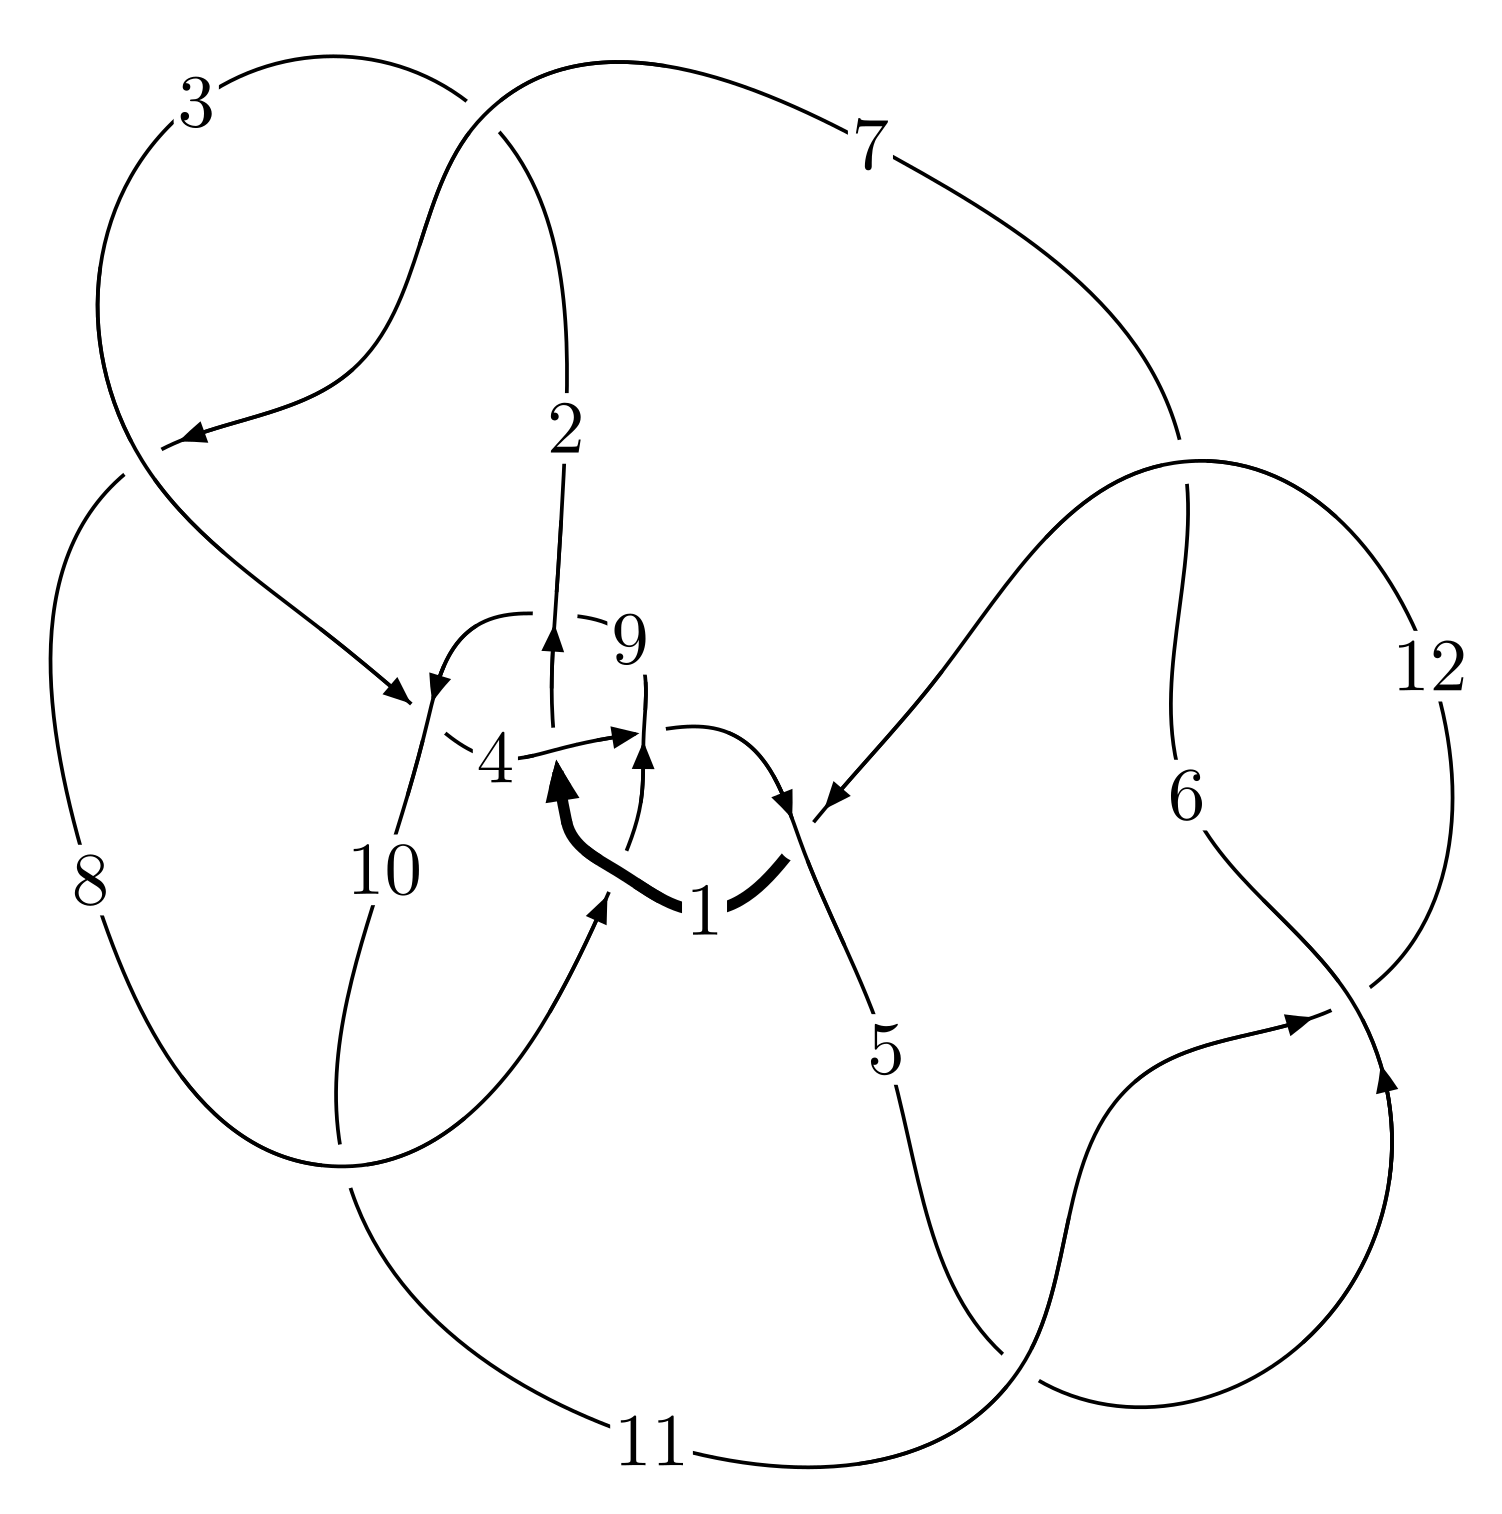
\includegraphics[width=112pt]{../../../GIT/diagram.site/Diagrams/png/1873_12a_1072.png}\\
\ \ \ A knot diagram\footnotemark}&
\allowdisplaybreaks
\textbf{Linearized knot diagam} \\
\cline{2-2}
 &
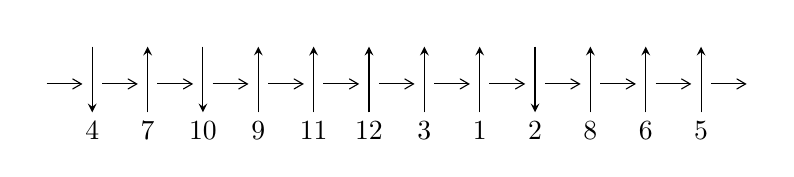
\begin{tikzpicture}[x=20pt, y=17pt]
	% nodes
	\node (C0) at (0, 0) {};
	\node (C1) at (1, 0) {};
	\node (C1U) at (1, +1) {};
	\node (C1D) at (1, -1) {4};

	\node (C2) at (2, 0) {};
	\node (C2U) at (2, +1) {};
	\node (C2D) at (2, -1) {7};

	\node (C3) at (3, 0) {};
	\node (C3U) at (3, +1) {};
	\node (C3D) at (3, -1) {10};

	\node (C4) at (4, 0) {};
	\node (C4U) at (4, +1) {};
	\node (C4D) at (4, -1) {9};

	\node (C5) at (5, 0) {};
	\node (C5U) at (5, +1) {};
	\node (C5D) at (5, -1) {11};

	\node (C6) at (6, 0) {};
	\node (C6U) at (6, +1) {};
	\node (C6D) at (6, -1) {12};

	\node (C7) at (7, 0) {};
	\node (C7U) at (7, +1) {};
	\node (C7D) at (7, -1) {3};

	\node (C8) at (8, 0) {};
	\node (C8U) at (8, +1) {};
	\node (C8D) at (8, -1) {1};

	\node (C9) at (9, 0) {};
	\node (C9U) at (9, +1) {};
	\node (C9D) at (9, -1) {2};

	\node (C10) at (10, 0) {};
	\node (C10U) at (10, +1) {};
	\node (C10D) at (10, -1) {8};

	\node (C11) at (11, 0) {};
	\node (C11U) at (11, +1) {};
	\node (C11D) at (11, -1) {6};

	\node (C12) at (12, 0) {};
	\node (C12U) at (12, +1) {};
	\node (C12D) at (12, -1) {5};
	\node (C13) at (13, 0) {};

	% arrows
	\draw[->,>={angle 60}]
	(C0) edge (C1) (C1) edge (C2) (C2) edge (C3) (C3) edge (C4) (C4) edge (C5) (C5) edge (C6) (C6) edge (C7) (C7) edge (C8) (C8) edge (C9) (C9) edge (C10) (C10) edge (C11) (C11) edge (C12) (C12) edge (C13) ;	\draw[->,>=stealth]
	(C1U) edge (C1D) (C2D) edge (C2U) (C3U) edge (C3D) (C4D) edge (C4U) (C5D) edge (C5U) (C6D) edge (C6U) (C7D) edge (C7U) (C8D) edge (C8U) (C9U) edge (C9D) (C10D) edge (C10U) (C11D) edge (C11U) (C12D) edge (C12U) ;
	\end{tikzpicture} \\
\hhline{~~} \\& 
\textbf{Solving Sequence} \\ \cline{2-2} 
 &
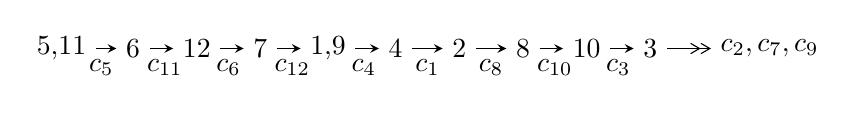
\begin{tikzpicture}[x=23pt, y=7pt]
	% node
	\node (A0) at (-1/8, 0) {5,11};
	\node (A1) at (1, 0) {6};
	\node (A2) at (2, 0) {12};
	\node (A3) at (3, 0) {7};
	\node (A4) at (65/16, 0) {1,9};
	\node (A5) at (41/8, 0) {4};
	\node (A6) at (49/8, 0) {2};
	\node (A7) at (57/8, 0) {8};
	\node (A8) at (65/8, 0) {10};
	\node (A9) at (73/8, 0) {3};
	\node (C1) at (1/2, -1) {$c_{5}$};
	\node (C2) at (3/2, -1) {$c_{11}$};
	\node (C3) at (5/2, -1) {$c_{6}$};
	\node (C4) at (7/2, -1) {$c_{12}$};
	\node (C5) at (37/8, -1) {$c_{4}$};
	\node (C6) at (45/8, -1) {$c_{1}$};
	\node (C7) at (53/8, -1) {$c_{8}$};
	\node (C8) at (61/8, -1) {$c_{10}$};
	\node (C9) at (69/8, -1) {$c_{3}$};
	\node (A10) at (11, 0) {$c_{2},c_{7},c_{9}$};

	% edge
	\draw[->,>=stealth]	
	(A0) edge (A1) (A1) edge (A2) (A2) edge (A3) (A3) edge (A4) (A4) edge (A5) (A5) edge (A6) (A6) edge (A7) (A7) edge (A8) (A8) edge (A9) ;
	\draw[->>,>={angle 60}]	
	(A9) edge (A10);
\end{tikzpicture} \\ 

\end{tabular} \\

\footnotetext{
The image of knot diagram is generated by the software ``\textbf{Draw programme}" developed by Andrew Bartholomew(\url{http://www.layer8.co.uk/maths/draw/index.htm\#Running-draw}), where we modified some parts for our purpose(\url{https://github.com/CATsTAILs/LinksPainter}).
}\phantom \\ \newline 
\centering \textbf{Ideals for irreducible components\footnotemark of $X_{\text{par}}$} 
 
\begin{align*}
I^u_{1}&=\langle 
6.92052\times10^{288} u^{153}+3.23848\times10^{289} u^{152}+\cdots+2.10567\times10^{289} b+9.66356\times10^{290},\\
\phantom{I^u_{1}}&\phantom{= \langle  }8.62661\times10^{290} u^{153}+5.83689\times10^{290} u^{152}+\cdots+1.03178\times10^{291} a+6.04649\times10^{292},\\
\phantom{I^u_{1}}&\phantom{= \langle  }u^{154}+u^{153}+\cdots+572 u+49\rangle \\
I^u_{2}&=\langle 
131 u^{33}+320 u^{32}+\cdots+29 b+254,\;39 u^{33}-154 u^{32}+\cdots+29 a+266,\;u^{34}-17 u^{32}+\cdots+8 u-1\rangle \\
\\
\end{align*}
\raggedright * 2 irreducible components of $\dim_{\mathbb{C}}=0$, with total 188 representations.\\
\footnotetext{All coefficients of polynomials are rational numbers. But the coefficients are sometimes approximated in decimal forms when there is not enough margin.}
\newpage
\renewcommand{\arraystretch}{1}
\centering \section*{I. $I^u_{1}= \langle 6.92\times10^{288} u^{153}+3.24\times10^{289} u^{152}+\cdots+2.11\times10^{289} b+9.66\times10^{290},\;8.63\times10^{290} u^{153}+5.84\times10^{290} u^{152}+\cdots+1.03\times10^{291} a+6.05\times10^{292},\;u^{154}+u^{153}+\cdots+572 u+49 \rangle$}
\flushleft \textbf{(i) Arc colorings}\\
\begin{tabular}{m{7pt} m{180pt} m{7pt} m{180pt} }
\flushright $a_{5}=$&$\begin{pmatrix}1\\0\end{pmatrix}$ \\
\flushright $a_{11}=$&$\begin{pmatrix}0\\u\end{pmatrix}$ \\
\flushright $a_{6}=$&$\begin{pmatrix}1\\- u^2\end{pmatrix}$ \\
\flushright $a_{12}=$&$\begin{pmatrix}u\\- u^3+u\end{pmatrix}$ \\
\flushright $a_{7}=$&$\begin{pmatrix}- u^2+1\\u^4-2 u^2\end{pmatrix}$ \\
\flushright $a_{1}=$&$\begin{pmatrix}- u^3+2 u\\- u^3+u\end{pmatrix}$ \\
\flushright $a_{9}=$&$\begin{pmatrix}-0.836091 u^{153}-0.565712 u^{152}+\cdots-584.309 u-58.6026\\-0.328661 u^{153}-1.53798 u^{152}+\cdots-489.932 u-45.8930\end{pmatrix}$ \\
\flushright $a_{4}=$&$\begin{pmatrix}0.112124 u^{153}+0.849429 u^{152}+\cdots+114.420 u+6.91067\\3.28754 u^{153}+0.173793 u^{152}+\cdots+1256.42 u+117.530\end{pmatrix}$ \\
\flushright $a_{2}=$&$\begin{pmatrix}-3.21081 u^{153}+1.99563 u^{152}+\cdots-1542.74 u-138.134\\-1.77663 u^{153}+2.17174 u^{152}+\cdots-523.262 u-44.5739\end{pmatrix}$ \\
\flushright $a_{8}=$&$\begin{pmatrix}3.89771 u^{153}-1.55113 u^{152}+\cdots+1539.52 u+140.027\\4.11046 u^{153}-3.67254 u^{152}+\cdots+823.579 u+74.3562\end{pmatrix}$ \\
\flushright $a_{10}=$&$\begin{pmatrix}-1.88491 u^{153}+0.809201 u^{152}+\cdots-968.956 u-100.031\\-4.29184 u^{153}+1.77326 u^{152}+\cdots-1544.83 u-143.097\end{pmatrix}$ \\
\flushright $a_{3}=$&$\begin{pmatrix}-4.27600 u^{153}+1.26668 u^{152}+\cdots-2150.52 u-195.941\\-7.94334 u^{153}+3.53383 u^{152}+\cdots-2913.25 u-262.894\end{pmatrix}$\\&\end{tabular}
\flushleft \textbf{(ii) Obstruction class $= -1$}\\~\\
\flushleft \textbf{(iii) Cusp Shapes $= -4.33212 u^{153}-0.684610 u^{152}+\cdots-1911.81 u-170.082$}\\~\\
\newpage\renewcommand{\arraystretch}{1}
\flushleft \textbf{(iv) u-Polynomials at the component}\newline \\
\begin{tabular}{m{50pt}|m{274pt}}
Crossings & \hspace{64pt}u-Polynomials at each crossing \\
\hline $$\begin{aligned}c_{1}\end{aligned}$$&$\begin{aligned}
&u^{154}-14 u^{153}+\cdots+40 u-1
\end{aligned}$\\
\hline $$\begin{aligned}c_{2},c_{7}\end{aligned}$$&$\begin{aligned}
&u^{154}+u^{153}+\cdots+1715 u-2401
\end{aligned}$\\
\hline $$\begin{aligned}c_{3}\end{aligned}$$&$\begin{aligned}
&u^{154}+u^{153}+\cdots-148813 u+30543
\end{aligned}$\\
\hline $$\begin{aligned}c_{4}\end{aligned}$$&$\begin{aligned}
&u^{154}+3 u^{153}+\cdots+6894 u+41
\end{aligned}$\\
\hline $$\begin{aligned}c_{5},c_{6},c_{11}\end{aligned}$$&$\begin{aligned}
&u^{154}+u^{153}+\cdots+572 u+49
\end{aligned}$\\
\hline $$\begin{aligned}c_{8}\end{aligned}$$&$\begin{aligned}
&u^{154}+7 u^{152}+\cdots+1316 u+187
\end{aligned}$\\
\hline $$\begin{aligned}c_{9}\end{aligned}$$&$\begin{aligned}
&u^{154}-3 u^{153}+\cdots+1930 u-83
\end{aligned}$\\
\hline $$\begin{aligned}c_{10}\end{aligned}$$&$\begin{aligned}
&u^{154}-7 u^{153}+\cdots+13536812 u-792892
\end{aligned}$\\
\hline $$\begin{aligned}c_{12}\end{aligned}$$&$\begin{aligned}
&u^{154}-6 u^{153}+\cdots-118592654 u-10006731
\end{aligned}$\\
\hline
\end{tabular}\\~\\
\newpage\renewcommand{\arraystretch}{1}
\flushleft \textbf{(v) Riley Polynomials at the component}\newline \\
\begin{tabular}{m{50pt}|m{274pt}}
Crossings & \hspace{64pt}Riley Polynomials at each crossing \\
\hline $$\begin{aligned}c_{1}\end{aligned}$$&$\begin{aligned}
&y^{154}+4 y^{153}+\cdots-96 y+1
\end{aligned}$\\
\hline $$\begin{aligned}c_{2},c_{7}\end{aligned}$$&$\begin{aligned}
&y^{154}-87 y^{153}+\cdots+38235925 y+5764801
\end{aligned}$\\
\hline $$\begin{aligned}c_{3}\end{aligned}$$&$\begin{aligned}
&y^{154}+33 y^{153}+\cdots+26474687753 y+932874849
\end{aligned}$\\
\hline $$\begin{aligned}c_{4}\end{aligned}$$&$\begin{aligned}
&y^{154}+19 y^{153}+\cdots-54147834 y+1681
\end{aligned}$\\
\hline $$\begin{aligned}c_{5},c_{6},c_{11}\end{aligned}$$&$\begin{aligned}
&y^{154}-137 y^{153}+\cdots+38356 y+2401
\end{aligned}$\\
\hline $$\begin{aligned}c_{8}\end{aligned}$$&$\begin{aligned}
&y^{154}+14 y^{153}+\cdots-2877044 y+34969
\end{aligned}$\\
\hline $$\begin{aligned}c_{9}\end{aligned}$$&$\begin{aligned}
&y^{154}+y^{153}+\cdots-2295640 y+6889
\end{aligned}$\\
\hline $$\begin{aligned}c_{10}\end{aligned}$$&$\begin{aligned}
&y^{154}-27 y^{153}+\cdots-308019410590464 y+628677723664
\end{aligned}$\\
\hline $$\begin{aligned}c_{12}\end{aligned}$$&$\begin{aligned}
&y^{154}+28 y^{153}+\cdots+1260521920984700 y+100134665306361
\end{aligned}$\\
\hline
\end{tabular}\\~\\
\newpage\flushleft \textbf{(vi) Complex Volumes and Cusp Shapes}
$$\begin{array}{c|c|c}  
\text{Solutions to }I^u_{1}& \I (\text{vol} + \sqrt{-1}CS) & \text{Cusp shape}\\
 \hline 
\begin{aligned}
u &= -0.927461 + 0.345607 I \\
a &= \phantom{-}0.571854 + 0.712390 I \\
b &= \phantom{-}0.698035 + 1.094410 I\end{aligned}
 & -0.40591 + 5.13144 I & \phantom{-0.000000 } 0 \\ \hline\begin{aligned}
u &= -0.927461 - 0.345607 I \\
a &= \phantom{-}0.571854 - 0.712390 I \\
b &= \phantom{-}0.698035 - 1.094410 I\end{aligned}
 & -0.40591 - 5.13144 I & \phantom{-0.000000 } 0 \\ \hline\begin{aligned}
u &= -1.010770 + 0.201290 I \\
a &= -0.460389 + 0.536054 I \\
b &= -0.168033 + 0.927326 I\end{aligned}
 & -1.90062 - 2.37239 I & \phantom{-0.000000 } 0 \\ \hline\begin{aligned}
u &= -1.010770 - 0.201290 I \\
a &= -0.460389 - 0.536054 I \\
b &= -0.168033 - 0.927326 I\end{aligned}
 & -1.90062 + 2.37239 I & \phantom{-0.000000 } 0 \\ \hline\begin{aligned}
u &= -0.746757 + 0.613077 I \\
a &= -1.227500 - 0.317196 I \\
b &= -0.816114 - 0.778786 I\end{aligned}
 & -0.94391 + 1.96290 I & \phantom{-0.000000 } 0 \\ \hline\begin{aligned}
u &= -0.746757 - 0.613077 I \\
a &= -1.227500 + 0.317196 I \\
b &= -0.816114 + 0.778786 I\end{aligned}
 & -0.94391 - 1.96290 I & \phantom{-0.000000 } 0 \\ \hline\begin{aligned}
u &= \phantom{-}0.862818 + 0.591068 I \\
a &= -0.045042 + 0.471122 I \\
b &= \phantom{-}0.042710 + 0.628655 I\end{aligned}
 & \phantom{-}0.85502 - 2.26604 I & \phantom{-0.000000 } 0 \\ \hline\begin{aligned}
u &= \phantom{-}0.862818 - 0.591068 I \\
a &= -0.045042 - 0.471122 I \\
b &= \phantom{-}0.042710 - 0.628655 I\end{aligned}
 & \phantom{-}0.85502 + 2.26604 I & \phantom{-0.000000 } 0 \\ \hline\begin{aligned}
u &= \phantom{-}0.483374 + 0.948619 I \\
a &= \phantom{-}0.803786 - 0.037733 I \\
b &= \phantom{-}0.595537 - 0.219838 I\end{aligned}
 & \phantom{-}1.84173 - 2.95635 I & \phantom{-0.000000 } 0 \\ \hline\begin{aligned}
u &= \phantom{-}0.483374 - 0.948619 I \\
a &= \phantom{-}0.803786 + 0.037733 I \\
b &= \phantom{-}0.595537 + 0.219838 I\end{aligned}
 & \phantom{-}1.84173 + 2.95635 I & \phantom{-0.000000 } 0\\
 \hline 
 \end{array}$$\newpage$$\begin{array}{c|c|c}  
\text{Solutions to }I^u_{1}& \I (\text{vol} + \sqrt{-1}CS) & \text{Cusp shape}\\
 \hline 
\begin{aligned}
u &= \phantom{-}0.952917 + 0.508089 I \\
a &= -0.976169 + 0.598595 I \\
b &= -0.91006 + 1.10434 I\end{aligned}
 & \phantom{-}2.83236 - 10.67170 I & \phantom{-0.000000 } 0 \\ \hline\begin{aligned}
u &= \phantom{-}0.952917 - 0.508089 I \\
a &= -0.976169 - 0.598595 I \\
b &= -0.91006 - 1.10434 I\end{aligned}
 & \phantom{-}2.83236 + 10.67170 I & \phantom{-0.000000 } 0 \\ \hline\begin{aligned}
u &= \phantom{-}0.886976 + 0.633968 I \\
a &= -0.344079 - 0.873989 I \\
b &= -0.733983 - 0.617344 I\end{aligned}
 & \phantom{-}3.27656 + 8.53519 I & \phantom{-0.000000 } 0 \\ \hline\begin{aligned}
u &= \phantom{-}0.886976 - 0.633968 I \\
a &= -0.344079 + 0.873989 I \\
b &= -0.733983 + 0.617344 I\end{aligned}
 & \phantom{-}3.27656 - 8.53519 I & \phantom{-0.000000 } 0 \\ \hline\begin{aligned}
u &= \phantom{-}0.281881 + 0.853471 I \\
a &= -0.391485 + 1.110960 I \\
b &= \phantom{-}0.251039 + 0.757686 I\end{aligned}
 & -0.97354 + 7.22662 I & \phantom{-0.000000 } 0 \\ \hline\begin{aligned}
u &= \phantom{-}0.281881 - 0.853471 I \\
a &= -0.391485 - 1.110960 I \\
b &= \phantom{-}0.251039 - 0.757686 I\end{aligned}
 & -0.97354 - 7.22662 I & \phantom{-0.000000 } 0 \\ \hline\begin{aligned}
u &= -0.086276 + 0.884667 I \\
a &= \phantom{-}0.143622 - 1.066430 I \\
b &= \phantom{-}0.121995 - 0.314126 I\end{aligned}
 & \phantom{-}0.672030 - 0.579524 I & \phantom{-0.000000 } 0 \\ \hline\begin{aligned}
u &= -0.086276 - 0.884667 I \\
a &= \phantom{-}0.143622 + 1.066430 I \\
b &= \phantom{-}0.121995 + 0.314126 I\end{aligned}
 & \phantom{-}0.672030 + 0.579524 I & \phantom{-0.000000 } 0 \\ \hline\begin{aligned}
u &= -1.105370 + 0.141236 I \\
a &= \phantom{-}0.587760 + 0.026600 I \\
b &= -0.810615 - 0.580088 I\end{aligned}
 & \phantom{-}5.03507 + 2.42489 I & \phantom{-0.000000 } 0 \\ \hline\begin{aligned}
u &= -1.105370 - 0.141236 I \\
a &= \phantom{-}0.587760 - 0.026600 I \\
b &= -0.810615 + 0.580088 I\end{aligned}
 & \phantom{-}5.03507 - 2.42489 I & \phantom{-0.000000 } 0\\
 \hline 
 \end{array}$$\newpage$$\begin{array}{c|c|c}  
\text{Solutions to }I^u_{1}& \I (\text{vol} + \sqrt{-1}CS) & \text{Cusp shape}\\
 \hline 
\begin{aligned}
u &= \phantom{-}0.242209 + 0.848590 I \\
a &= \phantom{-}0.36042 + 2.39047 I \\
b &= \phantom{-}0.98628 + 1.24227 I\end{aligned}
 & \phantom{-}0.6384 + 15.4605 I & \phantom{-0.000000 } 0 \\ \hline\begin{aligned}
u &= \phantom{-}0.242209 - 0.848590 I \\
a &= \phantom{-}0.36042 - 2.39047 I \\
b &= \phantom{-}0.98628 - 1.24227 I\end{aligned}
 & \phantom{-}0.6384 - 15.4605 I & \phantom{-0.000000 } 0 \\ \hline\begin{aligned}
u &= \phantom{-}1.053650 + 0.402796 I \\
a &= \phantom{-}0.915371 - 0.635809 I \\
b &= \phantom{-}0.656843 - 1.086280 I\end{aligned}
 & -0.562944 + 0.950486 I & \phantom{-0.000000 } 0 \\ \hline\begin{aligned}
u &= \phantom{-}1.053650 - 0.402796 I \\
a &= \phantom{-}0.915371 + 0.635809 I \\
b &= \phantom{-}0.656843 + 1.086280 I\end{aligned}
 & -0.562944 - 0.950486 I & \phantom{-0.000000 } 0 \\ \hline\begin{aligned}
u &= -0.306711 + 0.801519 I \\
a &= \phantom{-}0.51366 - 2.25002 I \\
b &= \phantom{-}0.97157 - 1.22070 I\end{aligned}
 & -2.36458 - 6.65719 I & \phantom{-0.000000 } 0 \\ \hline\begin{aligned}
u &= -0.306711 - 0.801519 I \\
a &= \phantom{-}0.51366 + 2.25002 I \\
b &= \phantom{-}0.97157 + 1.22070 I\end{aligned}
 & -2.36458 + 6.65719 I & \phantom{-0.000000 } 0 \\ \hline\begin{aligned}
u &= \phantom{-}0.159307 + 0.813312 I \\
a &= -0.39611 - 2.39837 I \\
b &= -0.81842 - 1.20208 I\end{aligned}
 & -3.30262 + 3.43339 I & \phantom{-0.000000 } 0 \\ \hline\begin{aligned}
u &= \phantom{-}0.159307 - 0.813312 I \\
a &= -0.39611 + 2.39837 I \\
b &= -0.81842 + 1.20208 I\end{aligned}
 & -3.30262 - 3.43339 I & \phantom{-0.000000 } 0 \\ \hline\begin{aligned}
u &= -0.781148 + 0.273232 I \\
a &= -0.190786 - 0.963389 I \\
b &= \phantom{-}0.569949 - 0.950312 I\end{aligned}
 & -0.17129 - 4.74542 I & \phantom{-0.000000 } 0 \\ \hline\begin{aligned}
u &= -0.781148 - 0.273232 I \\
a &= -0.190786 + 0.963389 I \\
b &= \phantom{-}0.569949 + 0.950312 I\end{aligned}
 & -0.17129 + 4.74542 I & \phantom{-0.000000 } 0\\
 \hline 
 \end{array}$$\newpage$$\begin{array}{c|c|c}  
\text{Solutions to }I^u_{1}& \I (\text{vol} + \sqrt{-1}CS) & \text{Cusp shape}\\
 \hline 
\begin{aligned}
u &= -0.216403 + 0.783124 I \\
a &= \phantom{-}0.02588 + 2.40282 I \\
b &= -0.82581 + 1.18258 I\end{aligned}
 & -2.63970 - 9.31367 I & \phantom{-0.000000 } 0 \\ \hline\begin{aligned}
u &= -0.216403 - 0.783124 I \\
a &= \phantom{-}0.02588 - 2.40282 I \\
b &= -0.82581 - 1.18258 I\end{aligned}
 & -2.63970 + 9.31367 I & \phantom{-0.000000 } 0 \\ \hline\begin{aligned}
u &= \phantom{-}0.575349 + 0.509126 I \\
a &= -0.572498 - 0.147197 I \\
b &= -0.616975 + 0.698394 I\end{aligned}
 & \phantom{-}4.36358 - 0.75106 I & \phantom{-0.000000 } 0 \\ \hline\begin{aligned}
u &= \phantom{-}0.575349 - 0.509126 I \\
a &= -0.572498 + 0.147197 I \\
b &= -0.616975 - 0.698394 I\end{aligned}
 & \phantom{-}4.36358 + 0.75106 I & \phantom{-0.000000 } 0 \\ \hline\begin{aligned}
u &= -1.217750 + 0.213144 I \\
a &= \phantom{-}2.32793 + 0.72652 I \\
b &= -0.015503 + 0.221781 I\end{aligned}
 & \phantom{-}3.36102 + 3.27740 I & \phantom{-0.000000 } 0 \\ \hline\begin{aligned}
u &= -1.217750 - 0.213144 I \\
a &= \phantom{-}2.32793 - 0.72652 I \\
b &= -0.015503 - 0.221781 I\end{aligned}
 & \phantom{-}3.36102 - 3.27740 I & \phantom{-0.000000 } 0 \\ \hline\begin{aligned}
u &= \phantom{-}1.210250 + 0.283808 I \\
a &= \phantom{-}0.350533 - 1.155720 I \\
b &= \phantom{-}0.318071 - 0.806501 I\end{aligned}
 & \phantom{-}0.88203 + 1.22872 I & \phantom{-0.000000 } 0 \\ \hline\begin{aligned}
u &= \phantom{-}1.210250 - 0.283808 I \\
a &= \phantom{-}0.350533 + 1.155720 I \\
b &= \phantom{-}0.318071 + 0.806501 I\end{aligned}
 & \phantom{-}0.88203 - 1.22872 I & \phantom{-0.000000 } 0 \\ \hline\begin{aligned}
u &= \phantom{-}0.056127 + 0.753685 I \\
a &= -1.00444 - 2.45512 I \\
b &= -1.20792 - 1.19422 I\end{aligned}
 & -2.03527 + 5.47232 I & \phantom{-0.000000 } 0 \\ \hline\begin{aligned}
u &= \phantom{-}0.056127 - 0.753685 I \\
a &= -1.00444 + 2.45512 I \\
b &= -1.20792 + 1.19422 I\end{aligned}
 & -2.03527 - 5.47232 I & \phantom{-0.000000 } 0\\
 \hline 
 \end{array}$$\newpage$$\begin{array}{c|c|c}  
\text{Solutions to }I^u_{1}& \I (\text{vol} + \sqrt{-1}CS) & \text{Cusp shape}\\
 \hline 
\begin{aligned}
u &= -1.242890 + 0.102023 I \\
a &= \phantom{-}0.67636 + 1.67439 I \\
b &= -1.59234 - 0.28562 I\end{aligned}
 & \phantom{-}5.07445 + 4.64277 I & \phantom{-0.000000 } 0 \\ \hline\begin{aligned}
u &= -1.242890 - 0.102023 I \\
a &= \phantom{-}0.67636 - 1.67439 I \\
b &= -1.59234 + 0.28562 I\end{aligned}
 & \phantom{-}5.07445 - 4.64277 I & \phantom{-0.000000 } 0 \\ \hline\begin{aligned}
u &= \phantom{-}0.054789 + 0.750359 I \\
a &= \phantom{-}0.14867 - 2.39554 I \\
b &= -0.373742 - 0.841489 I\end{aligned}
 & -2.62480 + 2.53088 I & \phantom{-0.000000 } 0 \\ \hline\begin{aligned}
u &= \phantom{-}0.054789 - 0.750359 I \\
a &= \phantom{-}0.14867 + 2.39554 I \\
b &= -0.373742 + 0.841489 I\end{aligned}
 & -2.62480 - 2.53088 I & \phantom{-0.000000 } 0 \\ \hline\begin{aligned}
u &= -0.177957 + 0.727362 I \\
a &= \phantom{-}0.103154 - 1.089410 I \\
b &= \phantom{-}0.958760 - 0.406201 I\end{aligned}
 & \phantom{-}2.52652 - 5.87194 I & \phantom{-0.000000 } 0 \\ \hline\begin{aligned}
u &= -0.177957 - 0.727362 I \\
a &= \phantom{-}0.103154 + 1.089410 I \\
b &= \phantom{-}0.958760 + 0.406201 I\end{aligned}
 & \phantom{-}2.52652 + 5.87194 I & \phantom{-0.000000 } 0 \\ \hline\begin{aligned}
u &= \phantom{-}1.213530 + 0.312350 I \\
a &= \phantom{-}0.883124 - 0.289434 I \\
b &= \phantom{-}1.03006 - 1.24793 I\end{aligned}
 & \phantom{-}1.50891 - 1.60866 I & \phantom{-0.000000 } 0 \\ \hline\begin{aligned}
u &= \phantom{-}1.213530 - 0.312350 I \\
a &= \phantom{-}0.883124 + 0.289434 I \\
b &= \phantom{-}1.03006 + 1.24793 I\end{aligned}
 & \phantom{-}1.50891 + 1.60866 I & \phantom{-0.000000 } 0 \\ \hline\begin{aligned}
u &= \phantom{-}0.031817 + 0.739153 I \\
a &= -0.57728 - 1.88386 I \\
b &= -0.408354 - 0.903776 I\end{aligned}
 & -2.37049 + 2.06375 I & \phantom{-0.000000 } 0 \\ \hline\begin{aligned}
u &= \phantom{-}0.031817 - 0.739153 I \\
a &= -0.57728 + 1.88386 I \\
b &= -0.408354 + 0.903776 I\end{aligned}
 & -2.37049 - 2.06375 I & \phantom{-0.000000 } 0\\
 \hline 
 \end{array}$$\newpage$$\begin{array}{c|c|c}  
\text{Solutions to }I^u_{1}& \I (\text{vol} + \sqrt{-1}CS) & \text{Cusp shape}\\
 \hline 
\begin{aligned}
u &= -0.237453 + 0.693513 I \\
a &= \phantom{-}0.926481 + 0.745244 I \\
b &= -0.125006 + 0.724198 I\end{aligned}
 & -4.13652 - 1.08958 I & \phantom{-0.000000 } 0 \\ \hline\begin{aligned}
u &= -0.237453 - 0.693513 I \\
a &= \phantom{-}0.926481 - 0.745244 I \\
b &= -0.125006 - 0.724198 I\end{aligned}
 & -4.13652 + 1.08958 I & \phantom{-0.000000 } 0 \\ \hline\begin{aligned}
u &= \phantom{-}1.248600 + 0.230177 I \\
a &= \phantom{-}1.025290 - 0.821994 I \\
b &= \phantom{-}0.010193 - 0.562579 I\end{aligned}
 & \phantom{-}1.37017 + 1.35061 I & \phantom{-0.000000 } 0 \\ \hline\begin{aligned}
u &= \phantom{-}1.248600 - 0.230177 I \\
a &= \phantom{-}1.025290 + 0.821994 I \\
b &= \phantom{-}0.010193 + 0.562579 I\end{aligned}
 & \phantom{-}1.37017 - 1.35061 I & \phantom{-0.000000 } 0 \\ \hline\begin{aligned}
u &= \phantom{-}0.324193 + 0.639588 I \\
a &= -0.37292 + 1.45768 I \\
b &= \phantom{-}0.794397 + 0.830062 I\end{aligned}
 & \phantom{-}3.58264 + 4.62489 I & \phantom{-}6.00000 - 6.36906 I \\ \hline\begin{aligned}
u &= \phantom{-}0.324193 - 0.639588 I \\
a &= -0.37292 - 1.45768 I \\
b &= \phantom{-}0.794397 - 0.830062 I\end{aligned}
 & \phantom{-}3.58264 - 4.62489 I & \phantom{-}6.00000 + 6.36906 I \\ \hline\begin{aligned}
u &= -1.274150 + 0.177617 I \\
a &= \phantom{-}1.96098 + 1.20727 I \\
b &= -0.279677 + 1.311780 I\end{aligned}
 & \phantom{-}6.16522 + 0.02142 I & \phantom{-0.000000 } 0 \\ \hline\begin{aligned}
u &= -1.274150 - 0.177617 I \\
a &= \phantom{-}1.96098 - 1.20727 I \\
b &= -0.279677 - 1.311780 I\end{aligned}
 & \phantom{-}6.16522 - 0.02142 I & \phantom{-0.000000 } 0 \\ \hline\begin{aligned}
u &= \phantom{-}1.249260 + 0.336649 I \\
a &= \phantom{-}0.725825 - 0.411585 I \\
b &= \phantom{-}0.188665 - 0.964491 I\end{aligned}
 & \phantom{-}1.45473 + 1.81129 I & \phantom{-0.000000 } 0 \\ \hline\begin{aligned}
u &= \phantom{-}1.249260 - 0.336649 I \\
a &= \phantom{-}0.725825 + 0.411585 I \\
b &= \phantom{-}0.188665 + 0.964491 I\end{aligned}
 & \phantom{-}1.45473 - 1.81129 I & \phantom{-0.000000 } 0\\
 \hline 
 \end{array}$$\newpage$$\begin{array}{c|c|c}  
\text{Solutions to }I^u_{1}& \I (\text{vol} + \sqrt{-1}CS) & \text{Cusp shape}\\
 \hline 
\begin{aligned}
u &= -1.243020 + 0.374967 I \\
a &= -0.400807 - 0.861821 I \\
b &= \phantom{-}0.103461 - 0.117002 I\end{aligned}
 & \phantom{-}4.27005 - 3.94623 I & \phantom{-0.000000 } 0 \\ \hline\begin{aligned}
u &= -1.243020 - 0.374967 I \\
a &= -0.400807 + 0.861821 I \\
b &= \phantom{-}0.103461 + 0.117002 I\end{aligned}
 & \phantom{-}4.27005 + 3.94623 I & \phantom{-0.000000 } 0 \\ \hline\begin{aligned}
u &= -1.287510 + 0.210580 I \\
a &= -0.834555 - 0.544861 I \\
b &= -0.79176 - 1.58697 I\end{aligned}
 & \phantom{-}1.82927 + 0.15971 I & \phantom{-0.000000 } 0 \\ \hline\begin{aligned}
u &= -1.287510 - 0.210580 I \\
a &= -0.834555 + 0.544861 I \\
b &= -0.79176 + 1.58697 I\end{aligned}
 & \phantom{-}1.82927 - 0.15971 I & \phantom{-0.000000 } 0 \\ \hline\begin{aligned}
u &= -1.285830 + 0.237322 I \\
a &= -0.465739 - 1.095680 I \\
b &= \phantom{-}0.221383 - 1.293260 I\end{aligned}
 & \phantom{-}1.55653 - 5.23786 I & \phantom{-0.000000 } 0 \\ \hline\begin{aligned}
u &= -1.285830 - 0.237322 I \\
a &= -0.465739 + 1.095680 I \\
b &= \phantom{-}0.221383 + 1.293260 I\end{aligned}
 & \phantom{-}1.55653 + 5.23786 I & \phantom{-0.000000 } 0 \\ \hline\begin{aligned}
u &= -1.289640 + 0.219047 I \\
a &= -0.67999 + 1.61686 I \\
b &= \phantom{-}0.194630 + 0.834773 I\end{aligned}
 & \phantom{-}0.19938 - 2.59730 I & \phantom{-0.000000 } 0 \\ \hline\begin{aligned}
u &= -1.289640 - 0.219047 I \\
a &= -0.67999 - 1.61686 I \\
b &= \phantom{-}0.194630 - 0.834773 I\end{aligned}
 & \phantom{-}0.19938 + 2.59730 I & \phantom{-0.000000 } 0 \\ \hline\begin{aligned}
u &= \phantom{-}1.299870 + 0.164751 I \\
a &= \phantom{-}0.080900 + 1.078540 I \\
b &= \phantom{-}1.273270 - 0.449311 I\end{aligned}
 & \phantom{-}3.08949 - 0.12155 I & \phantom{-0.000000 } 0 \\ \hline\begin{aligned}
u &= \phantom{-}1.299870 - 0.164751 I \\
a &= \phantom{-}0.080900 - 1.078540 I \\
b &= \phantom{-}1.273270 + 0.449311 I\end{aligned}
 & \phantom{-}3.08949 + 0.12155 I & \phantom{-0.000000 } 0\\
 \hline 
 \end{array}$$\newpage$$\begin{array}{c|c|c}  
\text{Solutions to }I^u_{1}& \I (\text{vol} + \sqrt{-1}CS) & \text{Cusp shape}\\
 \hline 
\begin{aligned}
u &= -0.245587 + 0.638390 I \\
a &= \phantom{-}2.53209 + 0.47153 I \\
b &= \phantom{-}1.67963 + 0.57965 I\end{aligned}
 & \phantom{-}2.56524 - 6.84359 I & \phantom{-}11.6477 + 10.2192 I \\ \hline\begin{aligned}
u &= -0.245587 - 0.638390 I \\
a &= \phantom{-}2.53209 - 0.47153 I \\
b &= \phantom{-}1.67963 - 0.57965 I\end{aligned}
 & \phantom{-}2.56524 + 6.84359 I & \phantom{-}11.6477 - 10.2192 I \\ \hline\begin{aligned}
u &= -0.005331 + 0.682509 I \\
a &= -0.79552 - 1.94814 I \\
b &= -0.237939 - 0.962473 I\end{aligned}
 & -2.38240 + 2.00040 I & \phantom{-}1.37127 - 4.02567 I \\ \hline\begin{aligned}
u &= -0.005331 - 0.682509 I \\
a &= -0.79552 + 1.94814 I \\
b &= -0.237939 + 0.962473 I\end{aligned}
 & -2.38240 - 2.00040 I & \phantom{-}1.37127 + 4.02567 I \\ \hline\begin{aligned}
u &= \phantom{-}1.317320 + 0.122192 I \\
a &= \phantom{-}0.429833 + 1.196260 I \\
b &= -0.580798 + 0.938573 I\end{aligned}
 & \phantom{-}6.45327 - 3.68927 I & \phantom{-0.000000 } 0 \\ \hline\begin{aligned}
u &= \phantom{-}1.317320 - 0.122192 I \\
a &= \phantom{-}0.429833 - 1.196260 I \\
b &= -0.580798 - 0.938573 I\end{aligned}
 & \phantom{-}6.45327 + 3.68927 I & \phantom{-0.000000 } 0 \\ \hline\begin{aligned}
u &= -1.289650 + 0.315303 I \\
a &= -1.29054 - 1.58533 I \\
b &= \phantom{-}0.357774 - 0.815738 I\end{aligned}
 & \phantom{-}1.56297 - 6.38698 I & \phantom{-0.000000 } 0 \\ \hline\begin{aligned}
u &= -1.289650 - 0.315303 I \\
a &= -1.29054 + 1.58533 I \\
b &= \phantom{-}0.357774 + 0.815738 I\end{aligned}
 & \phantom{-}1.56297 + 6.38698 I & \phantom{-0.000000 } 0 \\ \hline\begin{aligned}
u &= \phantom{-}1.305890 + 0.241641 I \\
a &= -1.84496 + 0.35076 I \\
b &= \phantom{-}0.342334 + 0.469472 I\end{aligned}
 & \phantom{-}0.49222 + 3.43137 I & \phantom{-0.000000 } 0 \\ \hline\begin{aligned}
u &= \phantom{-}1.305890 - 0.241641 I \\
a &= -1.84496 - 0.35076 I \\
b &= \phantom{-}0.342334 - 0.469472 I\end{aligned}
 & \phantom{-}0.49222 - 3.43137 I & \phantom{-0.000000 } 0\\
 \hline 
 \end{array}$$\newpage$$\begin{array}{c|c|c}  
\text{Solutions to }I^u_{1}& \I (\text{vol} + \sqrt{-1}CS) & \text{Cusp shape}\\
 \hline 
\begin{aligned}
u &= -0.099577 + 0.663417 I \\
a &= -1.49114 + 2.44767 I \\
b &= -0.076571 + 0.539335 I\end{aligned}
 & \phantom{-}0.01977 - 6.43626 I & \phantom{-}0.46155 + 8.86012 I \\ \hline\begin{aligned}
u &= -0.099577 - 0.663417 I \\
a &= -1.49114 - 2.44767 I \\
b &= -0.076571 - 0.539335 I\end{aligned}
 & \phantom{-}0.01977 + 6.43626 I & \phantom{-}0.46155 - 8.86012 I \\ \hline\begin{aligned}
u &= -1.292970 + 0.313632 I \\
a &= -0.69694 - 1.32877 I \\
b &= \phantom{-}0.593827 - 0.942249 I\end{aligned}
 & \phantom{-}1.77843 - 5.87906 I & \phantom{-0.000000 } 0 \\ \hline\begin{aligned}
u &= -1.292970 - 0.313632 I \\
a &= -0.69694 + 1.32877 I \\
b &= \phantom{-}0.593827 + 0.942249 I\end{aligned}
 & \phantom{-}1.77843 + 5.87906 I & \phantom{-0.000000 } 0 \\ \hline\begin{aligned}
u &= \phantom{-}1.317840 + 0.233872 I \\
a &= \phantom{-}1.57057 - 1.33587 I \\
b &= -1.22768 - 1.33972 I\end{aligned}
 & \phantom{-}2.24031 + 6.00533 I & \phantom{-0.000000 } 0 \\ \hline\begin{aligned}
u &= \phantom{-}1.317840 - 0.233872 I \\
a &= \phantom{-}1.57057 + 1.33587 I \\
b &= -1.22768 + 1.33972 I\end{aligned}
 & \phantom{-}2.24031 - 6.00533 I & \phantom{-0.000000 } 0 \\ \hline\begin{aligned}
u &= -1.304820 + 0.312787 I \\
a &= -1.17852 - 1.82056 I \\
b &= \phantom{-}1.37219 - 1.16236 I\end{aligned}
 & \phantom{-}2.22017 - 9.31903 I & \phantom{-0.000000 } 0 \\ \hline\begin{aligned}
u &= -1.304820 - 0.312787 I \\
a &= -1.17852 + 1.82056 I \\
b &= \phantom{-}1.37219 + 1.16236 I\end{aligned}
 & \phantom{-}2.22017 + 9.31903 I & \phantom{-0.000000 } 0 \\ \hline\begin{aligned}
u &= \phantom{-}1.332450 + 0.268889 I \\
a &= \phantom{-}0.30937 + 1.70442 I \\
b &= \phantom{-}0.053201 + 0.745514 I\end{aligned}
 & \phantom{-}4.53872 + 9.82699 I & \phantom{-0.000000 } 0 \\ \hline\begin{aligned}
u &= \phantom{-}1.332450 - 0.268889 I \\
a &= \phantom{-}0.30937 - 1.70442 I \\
b &= \phantom{-}0.053201 - 0.745514 I\end{aligned}
 & \phantom{-}4.53872 - 9.82699 I & \phantom{-0.000000 } 0\\
 \hline 
 \end{array}$$\newpage$$\begin{array}{c|c|c}  
\text{Solutions to }I^u_{1}& \I (\text{vol} + \sqrt{-1}CS) & \text{Cusp shape}\\
 \hline 
\begin{aligned}
u &= \phantom{-}1.341150 + 0.233736 I \\
a &= -1.42873 + 1.52710 I \\
b &= \phantom{-}0.31254 + 1.66322 I\end{aligned}
 & \phantom{-}7.11773 + 5.58500 I & \phantom{-0.000000 } 0 \\ \hline\begin{aligned}
u &= \phantom{-}1.341150 - 0.233736 I \\
a &= -1.42873 - 1.52710 I \\
b &= \phantom{-}0.31254 - 1.66322 I\end{aligned}
 & \phantom{-}7.11773 - 5.58500 I & \phantom{-0.000000 } 0 \\ \hline\begin{aligned}
u &= \phantom{-}1.353860 + 0.170918 I \\
a &= -0.054631 - 0.243033 I \\
b &= -0.88173 + 1.29481 I\end{aligned}
 & \phantom{-}7.90755 + 1.15105 I & \phantom{-0.000000 } 0 \\ \hline\begin{aligned}
u &= \phantom{-}1.353860 - 0.170918 I \\
a &= -0.054631 + 0.243033 I \\
b &= -0.88173 - 1.29481 I\end{aligned}
 & \phantom{-}7.90755 - 1.15105 I & \phantom{-0.000000 } 0 \\ \hline\begin{aligned}
u &= -0.475213 + 0.420175 I \\
a &= -0.52602 + 2.78054 I \\
b &= -1.06289 + 1.00975 I\end{aligned}
 & \phantom{-}3.53086 + 3.56258 I & \phantom{-}13.12101 - 4.27600 I \\ \hline\begin{aligned}
u &= -0.475213 - 0.420175 I \\
a &= -0.52602 - 2.78054 I \\
b &= -1.06289 - 1.00975 I\end{aligned}
 & \phantom{-}3.53086 - 3.56258 I & \phantom{-}13.12101 + 4.27600 I \\ \hline\begin{aligned}
u &= -1.365860 + 0.046277 I \\
a &= \phantom{-}1.156000 + 0.139591 I \\
b &= -0.952301 + 0.679905 I\end{aligned}
 & \phantom{-}6.84876 - 0.97616 I & \phantom{-0.000000 } 0 \\ \hline\begin{aligned}
u &= -1.365860 - 0.046277 I \\
a &= \phantom{-}1.156000 - 0.139591 I \\
b &= -0.952301 - 0.679905 I\end{aligned}
 & \phantom{-}6.84876 + 0.97616 I & \phantom{-0.000000 } 0 \\ \hline\begin{aligned}
u &= -1.342850 + 0.254146 I \\
a &= \phantom{-}0.174806 - 0.890178 I \\
b &= \phantom{-}1.286480 + 0.503519 I\end{aligned}
 & \phantom{-}4.39240 - 5.62462 I & \phantom{-0.000000 } 0 \\ \hline\begin{aligned}
u &= -1.342850 - 0.254146 I \\
a &= \phantom{-}0.174806 + 0.890178 I \\
b &= \phantom{-}1.286480 - 0.503519 I\end{aligned}
 & \phantom{-}4.39240 + 5.62462 I & \phantom{-0.000000 } 0\\
 \hline 
 \end{array}$$\newpage$$\begin{array}{c|c|c}  
\text{Solutions to }I^u_{1}& \I (\text{vol} + \sqrt{-1}CS) & \text{Cusp shape}\\
 \hline 
\begin{aligned}
u &= -0.622806 + 0.103056 I \\
a &= \phantom{-}0.733473 + 0.897374 I \\
b &= -0.646437 - 0.368074 I\end{aligned}
 & \phantom{-}4.79448 + 2.53540 I & \phantom{-}16.1502 - 3.0298 I \\ \hline\begin{aligned}
u &= -0.622806 - 0.103056 I \\
a &= \phantom{-}0.733473 - 0.897374 I \\
b &= -0.646437 + 0.368074 I\end{aligned}
 & \phantom{-}4.79448 - 2.53540 I & \phantom{-}16.1502 + 3.0298 I \\ \hline\begin{aligned}
u &= \phantom{-}0.151780 + 0.612265 I \\
a &= -1.58908 - 0.04517 I \\
b &= -1.125520 + 0.275882 I\end{aligned}
 & -0.31183 + 2.42662 I & \phantom{-}5.75230 - 5.56981 I \\ \hline\begin{aligned}
u &= \phantom{-}0.151780 - 0.612265 I \\
a &= -1.58908 + 0.04517 I \\
b &= -1.125520 - 0.275882 I\end{aligned}
 & -0.31183 - 2.42662 I & \phantom{-}5.75230 + 5.56981 I \\ \hline\begin{aligned}
u &= -0.033879 + 0.605996 I \\
a &= \phantom{-}1.91919 + 1.73905 I \\
b &= -0.218275 + 0.647464 I\end{aligned}
 & -3.73384 - 0.33721 I & \phantom{-}0.23306 - 4.01469 I \\ \hline\begin{aligned}
u &= -0.033879 - 0.605996 I \\
a &= \phantom{-}1.91919 - 1.73905 I \\
b &= -0.218275 - 0.647464 I\end{aligned}
 & -3.73384 + 0.33721 I & \phantom{-}0.23306 + 4.01469 I \\ \hline\begin{aligned}
u &= \phantom{-}1.366600 + 0.303640 I \\
a &= \phantom{-}1.018920 - 0.969860 I \\
b &= -1.036340 - 0.352772 I\end{aligned}
 & \phantom{-}7.41102 + 9.62053 I & \phantom{-0.000000 } 0 \\ \hline\begin{aligned}
u &= \phantom{-}1.366600 - 0.303640 I \\
a &= \phantom{-}1.018920 + 0.969860 I \\
b &= -1.036340 + 0.352772 I\end{aligned}
 & \phantom{-}7.41102 - 9.62053 I & \phantom{-0.000000 } 0 \\ \hline\begin{aligned}
u &= -1.361190 + 0.343416 I \\
a &= -1.06206 - 1.59674 I \\
b &= \phantom{-}0.93794 - 1.23067 I\end{aligned}
 & \phantom{-}1.49056 - 7.59816 I & \phantom{-0.000000 } 0 \\ \hline\begin{aligned}
u &= -1.361190 - 0.343416 I \\
a &= -1.06206 + 1.59674 I \\
b &= \phantom{-}0.93794 + 1.23067 I\end{aligned}
 & \phantom{-}1.49056 + 7.59816 I & \phantom{-0.000000 } 0\\
 \hline 
 \end{array}$$\newpage$$\begin{array}{c|c|c}  
\text{Solutions to }I^u_{1}& \I (\text{vol} + \sqrt{-1}CS) & \text{Cusp shape}\\
 \hline 
\begin{aligned}
u &= -0.042209 + 0.589562 I \\
a &= \phantom{-}0.50413 - 3.11062 I \\
b &= \phantom{-}0.97646 - 1.39737 I\end{aligned}
 & -2.06991 - 3.00529 I & \phantom{-}3.45797 + 1.71764 I \\ \hline\begin{aligned}
u &= -0.042209 - 0.589562 I \\
a &= \phantom{-}0.50413 + 3.11062 I \\
b &= \phantom{-}0.97646 + 1.39737 I\end{aligned}
 & -2.06991 + 3.00529 I & \phantom{-}3.45797 - 1.71764 I \\ \hline\begin{aligned}
u &= \phantom{-}1.411370 + 0.033932 I \\
a &= -1.018740 + 0.696446 I \\
b &= \phantom{-}0.801939 - 0.040281 I\end{aligned}
 & \phantom{-}11.03370 - 2.02041 I & \phantom{-0.000000 } 0 \\ \hline\begin{aligned}
u &= \phantom{-}1.411370 - 0.033932 I \\
a &= -1.018740 - 0.696446 I \\
b &= \phantom{-}0.801939 + 0.040281 I\end{aligned}
 & \phantom{-}11.03370 + 2.02041 I & \phantom{-0.000000 } 0 \\ \hline\begin{aligned}
u &= \phantom{-}1.39111 + 0.26505 I \\
a &= -0.693051 - 0.936409 I \\
b &= -1.98761 + 0.74541 I\end{aligned}
 & \phantom{-}7.76421 + 10.17900 I & \phantom{-0.000000 } 0 \\ \hline\begin{aligned}
u &= \phantom{-}1.39111 - 0.26505 I \\
a &= -0.693051 + 0.936409 I \\
b &= -1.98761 - 0.74541 I\end{aligned}
 & \phantom{-}7.76421 - 10.17900 I & \phantom{-0.000000 } 0 \\ \hline\begin{aligned}
u &= -0.097422 + 0.572014 I \\
a &= \phantom{-}0.04795 + 4.13629 I \\
b &= -0.13301 + 1.43433 I\end{aligned}
 & \phantom{-}2.53562 - 2.61678 I & \phantom{-}7.65323 + 3.37494 I \\ \hline\begin{aligned}
u &= -0.097422 - 0.572014 I \\
a &= \phantom{-}0.04795 - 4.13629 I \\
b &= -0.13301 - 1.43433 I\end{aligned}
 & \phantom{-}2.53562 + 2.61678 I & \phantom{-}7.65323 - 3.37494 I \\ \hline\begin{aligned}
u &= \phantom{-}1.37127 + 0.38317 I \\
a &= \phantom{-}0.411591 - 0.951983 I \\
b &= -0.288907 - 0.451225 I\end{aligned}
 & \phantom{-}5.31823 + 5.16393 I & \phantom{-0.000000 } 0 \\ \hline\begin{aligned}
u &= \phantom{-}1.37127 - 0.38317 I \\
a &= \phantom{-}0.411591 + 0.951983 I \\
b &= -0.288907 + 0.451225 I\end{aligned}
 & \phantom{-}5.31823 - 5.16393 I & \phantom{-0.000000 } 0\\
 \hline 
 \end{array}$$\newpage$$\begin{array}{c|c|c}  
\text{Solutions to }I^u_{1}& \I (\text{vol} + \sqrt{-1}CS) & \text{Cusp shape}\\
 \hline 
\begin{aligned}
u &= \phantom{-}1.39109 + 0.32342 I \\
a &= -1.27596 + 1.43874 I \\
b &= \phantom{-}0.91908 + 1.20609 I\end{aligned}
 & \phantom{-}2.45921 + 13.31740 I & \phantom{-0.000000 } 0 \\ \hline\begin{aligned}
u &= \phantom{-}1.39109 - 0.32342 I \\
a &= -1.27596 - 1.43874 I \\
b &= \phantom{-}0.91908 - 1.20609 I\end{aligned}
 & \phantom{-}2.45921 - 13.31740 I & \phantom{-0.000000 } 0 \\ \hline\begin{aligned}
u &= -1.40726 + 0.25675 I \\
a &= \phantom{-}1.21867 + 0.82570 I \\
b &= -0.927106 + 0.823962 I\end{aligned}
 & \phantom{-}9.05767 - 7.90642 I & \phantom{-0.000000 } 0 \\ \hline\begin{aligned}
u &= -1.40726 - 0.25675 I \\
a &= \phantom{-}1.21867 - 0.82570 I \\
b &= -0.927106 - 0.823962 I\end{aligned}
 & \phantom{-}9.05767 + 7.90642 I & \phantom{-0.000000 } 0 \\ \hline\begin{aligned}
u &= \phantom{-}1.41636 + 0.28687 I \\
a &= -0.813693 + 0.144583 I \\
b &= \phantom{-}0.314338 + 0.586404 I\end{aligned}
 & \phantom{-}1.18201 + 4.67102 I & \phantom{-0.000000 } 0 \\ \hline\begin{aligned}
u &= \phantom{-}1.41636 - 0.28687 I \\
a &= -0.813693 - 0.144583 I \\
b &= \phantom{-}0.314338 - 0.586404 I\end{aligned}
 & \phantom{-}1.18201 - 4.67102 I & \phantom{-0.000000 } 0 \\ \hline\begin{aligned}
u &= \phantom{-}1.44559 + 0.01179 I \\
a &= \phantom{-}0.613436 - 0.246027 I \\
b &= -0.840708 + 0.799253 I\end{aligned}
 & \phantom{-}6.80868 - 4.89337 I & \phantom{-0.000000 } 0 \\ \hline\begin{aligned}
u &= \phantom{-}1.44559 - 0.01179 I \\
a &= \phantom{-}0.613436 + 0.246027 I \\
b &= -0.840708 - 0.799253 I\end{aligned}
 & \phantom{-}6.80868 + 4.89337 I & \phantom{-0.000000 } 0 \\ \hline\begin{aligned}
u &= \phantom{-}1.44646 + 0.13225 I \\
a &= -0.687178 + 1.052560 I \\
b &= \phantom{-}1.38508 + 1.66807 I\end{aligned}
 & \phantom{-}9.69626 - 1.57200 I & \phantom{-0.000000 } 0 \\ \hline\begin{aligned}
u &= \phantom{-}1.44646 - 0.13225 I \\
a &= -0.687178 - 1.052560 I \\
b &= \phantom{-}1.38508 - 1.66807 I\end{aligned}
 & \phantom{-}9.69626 + 1.57200 I & \phantom{-0.000000 } 0\\
 \hline 
 \end{array}$$\newpage$$\begin{array}{c|c|c}  
\text{Solutions to }I^u_{1}& \I (\text{vol} + \sqrt{-1}CS) & \text{Cusp shape}\\
 \hline 
\begin{aligned}
u &= -1.41225 + 0.35137 I \\
a &= \phantom{-}1.04127 + 1.59289 I \\
b &= -1.07034 + 1.30531 I\end{aligned}
 & \phantom{-}5.8916 - 19.7868 I & \phantom{-0.000000 } 0 \\ \hline\begin{aligned}
u &= -1.41225 - 0.35137 I \\
a &= \phantom{-}1.04127 - 1.59289 I \\
b &= -1.07034 - 1.30531 I\end{aligned}
 & \phantom{-}5.8916 + 19.7868 I & \phantom{-0.000000 } 0 \\ \hline\begin{aligned}
u &= \phantom{-}1.43168 + 0.32493 I \\
a &= \phantom{-}0.81916 - 1.50021 I \\
b &= -1.14887 - 1.40173 I\end{aligned}
 & \phantom{-}3.16978 + 10.74400 I & \phantom{-0.000000 } 0 \\ \hline\begin{aligned}
u &= \phantom{-}1.43168 - 0.32493 I \\
a &= \phantom{-}0.81916 + 1.50021 I \\
b &= -1.14887 + 1.40173 I\end{aligned}
 & \phantom{-}3.16978 - 10.74400 I & \phantom{-0.000000 } 0 \\ \hline\begin{aligned}
u &= -1.42760 + 0.34999 I \\
a &= \phantom{-}0.800137 + 0.665205 I \\
b &= -0.436085 + 0.765528 I\end{aligned}
 & \phantom{-}4.45777 - 11.57030 I & \phantom{-0.000000 } 0 \\ \hline\begin{aligned}
u &= -1.42760 - 0.34999 I \\
a &= \phantom{-}0.800137 - 0.665205 I \\
b &= -0.436085 - 0.765528 I\end{aligned}
 & \phantom{-}4.45777 + 11.57030 I & \phantom{-0.000000 } 0 \\ \hline\begin{aligned}
u &= -1.47194\phantom{ +0.000000I} \\
a &= \phantom{-}0.152404\phantom{ +0.000000I} \\
b &= -1.95358\phantom{ +0.000000I}\end{aligned}
 & \phantom{-}7.22309\phantom{ +0.000000I} & \phantom{-0.000000 } 0 \\ \hline\begin{aligned}
u &= \phantom{-}0.477522 + 0.201537 I \\
a &= -0.335158 + 1.151520 I \\
b &= \phantom{-}0.733536 + 0.515260 I\end{aligned}
 & \phantom{-}1.221320 + 0.185595 I & \phantom{-}10.16950 - 2.00322 I \\ \hline\begin{aligned}
u &= \phantom{-}0.477522 - 0.201537 I \\
a &= -0.335158 - 1.151520 I \\
b &= \phantom{-}0.733536 - 0.515260 I\end{aligned}
 & \phantom{-}1.221320 - 0.185595 I & \phantom{-}10.16950 + 2.00322 I \\ \hline\begin{aligned}
u &= -1.48224 + 0.10932 I \\
a &= -0.268936 - 0.479318 I \\
b &= \phantom{-}0.682969 + 0.376562 I\end{aligned}
 & \phantom{-}11.12170 - 1.32657 I & \phantom{-0.000000 } 0\\
 \hline 
 \end{array}$$\newpage$$\begin{array}{c|c|c}  
\text{Solutions to }I^u_{1}& \I (\text{vol} + \sqrt{-1}CS) & \text{Cusp shape}\\
 \hline 
\begin{aligned}
u &= -1.48224 - 0.10932 I \\
a &= -0.268936 + 0.479318 I \\
b &= \phantom{-}0.682969 - 0.376562 I\end{aligned}
 & \phantom{-}11.12170 + 1.32657 I & \phantom{-0.000000 } 0 \\ \hline\begin{aligned}
u &= -1.48920 + 0.22849 I \\
a &= \phantom{-}0.038534 + 0.481933 I \\
b &= -1.006450 + 0.213522 I\end{aligned}
 & \phantom{-}8.65591 - 0.95099 I & \phantom{-0.000000 } 0 \\ \hline\begin{aligned}
u &= -1.48920 - 0.22849 I \\
a &= \phantom{-}0.038534 - 0.481933 I \\
b &= -1.006450 - 0.213522 I\end{aligned}
 & \phantom{-}8.65591 + 0.95099 I & \phantom{-0.000000 } 0 \\ \hline\begin{aligned}
u &= \phantom{-}0.485422\phantom{ +0.000000I} \\
a &= \phantom{-}0.280440\phantom{ +0.000000I} \\
b &= \phantom{-}0.634586\phantom{ +0.000000I}\end{aligned}
 & \phantom{-}0.857296\phantom{ +0.000000I} & \phantom{-}12.0490\phantom{ +0.000000I} \\ \hline\begin{aligned}
u &= -1.51774 + 0.04528 I \\
a &= -0.387912 - 0.125330 I \\
b &= \phantom{-}1.158590 - 0.797595 I\end{aligned}
 & \phantom{-}11.5235 - 10.1880 I & \phantom{-0.000000 } 0 \\ \hline\begin{aligned}
u &= -1.51774 - 0.04528 I \\
a &= -0.387912 + 0.125330 I \\
b &= \phantom{-}1.158590 + 0.797595 I\end{aligned}
 & \phantom{-}11.5235 + 10.1880 I & \phantom{-0.000000 } 0 \\ \hline\begin{aligned}
u &= -0.333734 + 0.345049 I \\
a &= -1.76614 - 0.05989 I \\
b &= -0.577943 - 0.763081 I\end{aligned}
 & -1.45421 + 1.78453 I & -0.112248 - 1.219299 I \\ \hline\begin{aligned}
u &= -0.333734 - 0.345049 I \\
a &= -1.76614 + 0.05989 I \\
b &= -0.577943 + 0.763081 I\end{aligned}
 & -1.45421 - 1.78453 I & -0.112248 + 1.219299 I \\ \hline\begin{aligned}
u &= -0.189391 + 0.426079 I \\
a &= \phantom{-}0.525304 + 1.248360 I \\
b &= \phantom{-}0.682716 + 1.034730 I\end{aligned}
 & \phantom{-}3.03965 + 1.07983 I & \phantom{-}8.05417 + 4.35038 I \\ \hline\begin{aligned}
u &= -0.189391 - 0.426079 I \\
a &= \phantom{-}0.525304 - 1.248360 I \\
b &= \phantom{-}0.682716 - 1.034730 I\end{aligned}
 & \phantom{-}3.03965 - 1.07983 I & \phantom{-}8.05417 - 4.35038 I\\
 \hline 
 \end{array}$$\newpage$$\begin{array}{c|c|c}  
\text{Solutions to }I^u_{1}& \I (\text{vol} + \sqrt{-1}CS) & \text{Cusp shape}\\
 \hline 
\begin{aligned}
u &= \phantom{-}1.56975\phantom{ +0.000000I} \\
a &= \phantom{-}0.142767\phantom{ +0.000000I} \\
b &= \phantom{-}1.55545\phantom{ +0.000000I}\end{aligned}
 & \phantom{-}7.63894\phantom{ +0.000000I} & \phantom{-0.000000 } 0 \\ \hline\begin{aligned}
u &= -1.68430\phantom{ +0.000000I} \\
a &= -0.0947263\phantom{ +0.000000I} \\
b &= -0.00556291\phantom{ +0.000000I}\end{aligned}
 & \phantom{-}10.1752\phantom{ +0.000000I} & \phantom{-0.000000 } 0 \\ \hline\begin{aligned}
u &= -0.129828 + 0.157428 I \\
a &= -3.05094 + 4.63072 I \\
b &= \phantom{-}0.764905 + 0.606177 I\end{aligned}
 & \phantom{-}2.01233 + 4.97977 I & \phantom{-}8.23013 - 5.61565 I \\ \hline\begin{aligned}
u &= -0.129828 - 0.157428 I \\
a &= -3.05094 - 4.63072 I \\
b &= \phantom{-}0.764905 - 0.606177 I\end{aligned}
 & \phantom{-}2.01233 - 4.97977 I & \phantom{-}8.23013 + 5.61565 I\\
 \hline 
 \end{array}$$\newpage\newpage\renewcommand{\arraystretch}{1}
\centering \section*{II. $I^u_{2}= \langle 131 u^{33}+320 u^{32}+\cdots+29 b+254,\;39 u^{33}-154 u^{32}+\cdots+29 a+266,\;u^{34}-17 u^{32}+\cdots+8 u-1 \rangle$}
\flushleft \textbf{(i) Arc colorings}\\
\begin{tabular}{m{7pt} m{180pt} m{7pt} m{180pt} }
\flushright $a_{5}=$&$\begin{pmatrix}1\\0\end{pmatrix}$ \\
\flushright $a_{11}=$&$\begin{pmatrix}0\\u\end{pmatrix}$ \\
\flushright $a_{6}=$&$\begin{pmatrix}1\\- u^2\end{pmatrix}$ \\
\flushright $a_{12}=$&$\begin{pmatrix}u\\- u^3+u\end{pmatrix}$ \\
\flushright $a_{7}=$&$\begin{pmatrix}- u^2+1\\u^4-2 u^2\end{pmatrix}$ \\
\flushright $a_{1}=$&$\begin{pmatrix}- u^3+2 u\\- u^3+u\end{pmatrix}$ \\
\flushright $a_{9}=$&$\begin{pmatrix}-1.34483 u^{33}+5.31034 u^{32}+\cdots+12.7931 u-9.17241\\-4.51724 u^{33}-11.0345 u^{32}+\cdots+60.6897 u-8.75862\end{pmatrix}$ \\
\flushright $a_{4}=$&$\begin{pmatrix}9.86207 u^{33}+18.7241 u^{32}+\cdots-128.483 u+17.9310\\-11.1724 u^{33}-9.34483 u^{32}+\cdots+40.8966 u-6.58621\end{pmatrix}$ \\
\flushright $a_{2}=$&$\begin{pmatrix}-0.448276 u^{33}+3.10345 u^{32}+\cdots-27.0690 u+9.27586\\-2 u^{33}- u^{32}+\cdots+u+1\end{pmatrix}$ \\
\flushright $a_{8}=$&$\begin{pmatrix}-1.34483 u^{33}+4.31034 u^{32}+\cdots+18.7931 u-10.1724\\-4.51724 u^{33}-13.0345 u^{32}+\cdots+67.6897 u-9.75862\end{pmatrix}$ \\
\flushright $a_{10}=$&$\begin{pmatrix}5.24138 u^{33}+1.48276 u^{32}+\cdots+50.3448 u-15.3793\\-10.5172 u^{33}-7.03448 u^{32}+\cdots+15.6897 u-3.75862\end{pmatrix}$ \\
\flushright $a_{3}=$&$\begin{pmatrix}-1.20690 u^{33}+1.58621 u^{32}+\cdots-21.7241 u+9.89655\\0.689655 u^{33}-4.62069 u^{32}+\cdots+23.4138 u-1.65517\end{pmatrix}$\\&\end{tabular}
\flushleft \textbf{(ii) Obstruction class $= 1$}\\~\\
\flushleft \textbf{(iii) Cusp Shapes $= \frac{1041}{29} u^{33}+\frac{1009}{29} u^{32}+\cdots-\frac{3998}{29} u+\frac{912}{29}$}\\~\\
\newpage\renewcommand{\arraystretch}{1}
\flushleft \textbf{(iv) u-Polynomials at the component}\newline \\
\begin{tabular}{m{50pt}|m{274pt}}
Crossings & \hspace{64pt}u-Polynomials at each crossing \\
\hline $$\begin{aligned}c_{1}\end{aligned}$$&$\begin{aligned}
&u^{34}-3 u^{33}+\cdots+2 u^2-1
\end{aligned}$\\
\hline $$\begin{aligned}c_{2}\end{aligned}$$&$\begin{aligned}
&u^{34}-8 u^{32}+\cdots+u+1
\end{aligned}$\\
\hline $$\begin{aligned}c_{3}\end{aligned}$$&$\begin{aligned}
&u^{34}-2 u^{32}+\cdots- u-1
\end{aligned}$\\
\hline $$\begin{aligned}c_{4}\end{aligned}$$&$\begin{aligned}
&u^{34}+u^{32}+\cdots-4 u-1
\end{aligned}$\\
\hline $$\begin{aligned}c_{5},c_{6}\end{aligned}$$&$\begin{aligned}
&u^{34}-17 u^{32}+\cdots+8 u-1
\end{aligned}$\\
\hline $$\begin{aligned}c_{7}\end{aligned}$$&$\begin{aligned}
&u^{34}-8 u^{32}+\cdots- u+1
\end{aligned}$\\
\hline $$\begin{aligned}c_{8}\end{aligned}$$&$\begin{aligned}
&u^{34}+u^{33}+\cdots+4 u^2+1
\end{aligned}$\\
\hline $$\begin{aligned}c_{9}\end{aligned}$$&$\begin{aligned}
&u^{34}+4 u^{32}+\cdots+4 u+1
\end{aligned}$\\
\hline $$\begin{aligned}c_{10}\end{aligned}$$&$\begin{aligned}
&u^{34}-12 u^{33}+\cdots-56 u+4
\end{aligned}$\\
\hline $$\begin{aligned}c_{11}\end{aligned}$$&$\begin{aligned}
&u^{34}-17 u^{32}+\cdots-8 u-1
\end{aligned}$\\
\hline $$\begin{aligned}c_{12}\end{aligned}$$&$\begin{aligned}
&u^{34}+3 u^{33}+\cdots-8 u-1
\end{aligned}$\\
\hline
\end{tabular}\\~\\
\newpage\renewcommand{\arraystretch}{1}
\flushleft \textbf{(v) Riley Polynomials at the component}\newline \\
\begin{tabular}{m{50pt}|m{274pt}}
Crossings & \hspace{64pt}Riley Polynomials at each crossing \\
\hline $$\begin{aligned}c_{1}\end{aligned}$$&$\begin{aligned}
&y^{34}-13 y^{33}+\cdots-4 y+1
\end{aligned}$\\
\hline $$\begin{aligned}c_{2},c_{7}\end{aligned}$$&$\begin{aligned}
&y^{34}-16 y^{33}+\cdots-31 y+1
\end{aligned}$\\
\hline $$\begin{aligned}c_{3}\end{aligned}$$&$\begin{aligned}
&y^{34}-4 y^{33}+\cdots+21 y+1
\end{aligned}$\\
\hline $$\begin{aligned}c_{4}\end{aligned}$$&$\begin{aligned}
&y^{34}+2 y^{33}+\cdots-22 y+1
\end{aligned}$\\
\hline $$\begin{aligned}c_{5},c_{6},c_{11}\end{aligned}$$&$\begin{aligned}
&y^{34}-34 y^{33}+\cdots-32 y+1
\end{aligned}$\\
\hline $$\begin{aligned}c_{8}\end{aligned}$$&$\begin{aligned}
&y^{34}+21 y^{33}+\cdots+8 y+1
\end{aligned}$\\
\hline $$\begin{aligned}c_{9}\end{aligned}$$&$\begin{aligned}
&y^{34}+8 y^{33}+\cdots+4 y+1
\end{aligned}$\\
\hline $$\begin{aligned}c_{10}\end{aligned}$$&$\begin{aligned}
&y^{34}+4 y^{33}+\cdots+80 y+16
\end{aligned}$\\
\hline $$\begin{aligned}c_{12}\end{aligned}$$&$\begin{aligned}
&y^{34}-9 y^{33}+\cdots-28 y+1
\end{aligned}$\\
\hline
\end{tabular}\\~\\
\newpage\flushleft \textbf{(vi) Complex Volumes and Cusp Shapes}
$$\begin{array}{c|c|c}  
\text{Solutions to }I^u_{2}& \I (\text{vol} + \sqrt{-1}CS) & \text{Cusp shape}\\
 \hline 
\begin{aligned}
u &= \phantom{-}0.526308 + 0.787564 I \\
a &= \phantom{-}0.864342 + 0.181925 I \\
b &= \phantom{-}0.485578 - 0.148400 I\end{aligned}
 & \phantom{-}1.52448 - 2.92080 I & \phantom{-}0.91674 + 5.58965 I \\ \hline\begin{aligned}
u &= \phantom{-}0.526308 - 0.787564 I \\
a &= \phantom{-}0.864342 - 0.181925 I \\
b &= \phantom{-}0.485578 + 0.148400 I\end{aligned}
 & \phantom{-}1.52448 + 2.92080 I & \phantom{-}0.91674 - 5.58965 I \\ \hline\begin{aligned}
u &= -1.164280 + 0.179890 I \\
a &= -0.684467 - 1.050570 I \\
b &= \phantom{-}0.457760 - 1.201170 I\end{aligned}
 & \phantom{-}1.26287 - 3.90402 I & \phantom{-}7.85607 + 2.42666 I \\ \hline\begin{aligned}
u &= -1.164280 - 0.179890 I \\
a &= -0.684467 + 1.050570 I \\
b &= \phantom{-}0.457760 + 1.201170 I\end{aligned}
 & \phantom{-}1.26287 + 3.90402 I & \phantom{-}7.85607 - 2.42666 I \\ \hline\begin{aligned}
u &= \phantom{-}1.155990 + 0.284819 I \\
a &= -0.22935 - 1.75427 I \\
b &= -0.622169 - 0.514867 I\end{aligned}
 & \phantom{-}3.49748 + 6.80335 I & \phantom{-}11.5376 - 8.2096 I \\ \hline\begin{aligned}
u &= \phantom{-}1.155990 - 0.284819 I \\
a &= -0.22935 + 1.75427 I \\
b &= -0.622169 + 0.514867 I\end{aligned}
 & \phantom{-}3.49748 - 6.80335 I & \phantom{-}11.5376 + 8.2096 I \\ \hline\begin{aligned}
u &= -1.195910 + 0.244747 I \\
a &= -1.075200 - 0.238234 I \\
b &= -0.89137 - 1.41358 I\end{aligned}
 & \phantom{-}0.732461 + 0.915441 I & \phantom{-}4.04182 - 1.39990 I \\ \hline\begin{aligned}
u &= -1.195910 - 0.244747 I \\
a &= -1.075200 + 0.238234 I \\
b &= -0.89137 + 1.41358 I\end{aligned}
 & \phantom{-}0.732461 - 0.915441 I & \phantom{-}4.04182 + 1.39990 I \\ \hline\begin{aligned}
u &= \phantom{-}1.220150 + 0.177222 I \\
a &= -1.284560 + 0.381957 I \\
b &= \phantom{-}0.956591 - 0.459125 I\end{aligned}
 & \phantom{-}4.33078 - 3.58495 I & \phantom{-}10.35085 + 5.27900 I \\ \hline\begin{aligned}
u &= \phantom{-}1.220150 - 0.177222 I \\
a &= -1.284560 - 0.381957 I \\
b &= \phantom{-}0.956591 + 0.459125 I\end{aligned}
 & \phantom{-}4.33078 + 3.58495 I & \phantom{-}10.35085 - 5.27900 I\\
 \hline 
 \end{array}$$\newpage$$\begin{array}{c|c|c}  
\text{Solutions to }I^u_{2}& \I (\text{vol} + \sqrt{-1}CS) & \text{Cusp shape}\\
 \hline 
\begin{aligned}
u &= -0.532052 + 0.526498 I \\
a &= -1.51021 - 0.47276 I \\
b &= -0.783339 - 0.789584 I\end{aligned}
 & -0.69563 + 1.42318 I & \phantom{-}10.44389 + 3.14665 I \\ \hline\begin{aligned}
u &= -0.532052 - 0.526498 I \\
a &= -1.51021 + 0.47276 I \\
b &= -0.783339 + 0.789584 I\end{aligned}
 & -0.69563 - 1.42318 I & \phantom{-}10.44389 - 3.14665 I \\ \hline\begin{aligned}
u &= -0.131665 + 0.732350 I \\
a &= \phantom{-}0.82839 - 2.67661 I \\
b &= \phantom{-}1.09485 - 1.31813 I\end{aligned}
 & -2.39868 - 4.42435 I & \phantom{-}4.23991 + 5.65394 I \\ \hline\begin{aligned}
u &= -0.131665 - 0.732350 I \\
a &= \phantom{-}0.82839 + 2.67661 I \\
b &= \phantom{-}1.09485 + 1.31813 I\end{aligned}
 & -2.39868 + 4.42435 I & \phantom{-}4.23991 - 5.65394 I \\ \hline\begin{aligned}
u &= -1.241240 + 0.212874 I \\
a &= \phantom{-}0.81651 - 1.44311 I \\
b &= -0.144983 - 0.774871 I\end{aligned}
 & -0.17471 - 2.07205 I & \phantom{-}1.71001 - 2.67417 I \\ \hline\begin{aligned}
u &= -1.241240 - 0.212874 I \\
a &= \phantom{-}0.81651 + 1.44311 I \\
b &= -0.144983 + 0.774871 I\end{aligned}
 & -0.17471 + 2.07205 I & \phantom{-}1.71001 + 2.67417 I \\ \hline\begin{aligned}
u &= \phantom{-}1.301910 + 0.008397 I \\
a &= -1.55655 - 0.33198 I \\
b &= \phantom{-}0.721682 + 0.892920 I\end{aligned}
 & \phantom{-}7.30584 + 2.09187 I & \phantom{-}16.7276 - 4.2341 I \\ \hline\begin{aligned}
u &= \phantom{-}1.301910 - 0.008397 I \\
a &= -1.55655 + 0.33198 I \\
b &= \phantom{-}0.721682 - 0.892920 I\end{aligned}
 & \phantom{-}7.30584 - 2.09187 I & \phantom{-}16.7276 + 4.2341 I \\ \hline\begin{aligned}
u &= \phantom{-}0.196510 + 0.635568 I \\
a &= -0.400631 - 0.095481 I \\
b &= -0.978314 - 0.259772 I\end{aligned}
 & \phantom{-}1.32286 + 6.33923 I & \phantom{-}5.25953 - 8.51173 I \\ \hline\begin{aligned}
u &= \phantom{-}0.196510 - 0.635568 I \\
a &= -0.400631 + 0.095481 I \\
b &= -0.978314 + 0.259772 I\end{aligned}
 & \phantom{-}1.32286 - 6.33923 I & \phantom{-}5.25953 + 8.51173 I\\
 \hline 
 \end{array}$$\newpage$$\begin{array}{c|c|c}  
\text{Solutions to }I^u_{2}& \I (\text{vol} + \sqrt{-1}CS) & \text{Cusp shape}\\
 \hline 
\begin{aligned}
u &= -0.143113 + 0.629395 I \\
a &= -1.57327 - 0.85037 I \\
b &= \phantom{-}0.181906 - 0.605964 I\end{aligned}
 & -3.53657 - 0.88192 I & \phantom{-}7.59270 + 6.75780 I \\ \hline\begin{aligned}
u &= -0.143113 - 0.629395 I \\
a &= -1.57327 + 0.85037 I \\
b &= \phantom{-}0.181906 + 0.605964 I\end{aligned}
 & -3.53657 + 0.88192 I & \phantom{-}7.59270 - 6.75780 I \\ \hline\begin{aligned}
u &= \phantom{-}1.346010 + 0.318175 I \\
a &= \phantom{-}1.09335 - 1.73483 I \\
b &= -1.22377 - 1.32062 I\end{aligned}
 & \phantom{-}2.26293 + 8.25380 I & \phantom{-0.000000 } 0 \\ \hline\begin{aligned}
u &= \phantom{-}1.346010 - 0.318175 I \\
a &= \phantom{-}1.09335 + 1.73483 I \\
b &= -1.22377 + 1.32062 I\end{aligned}
 & \phantom{-}2.26293 - 8.25380 I & \phantom{-0.000000 } 0 \\ \hline\begin{aligned}
u &= \phantom{-}1.375750 + 0.282089 I \\
a &= \phantom{-}1.046070 - 0.193076 I \\
b &= -0.302945 - 0.455018 I\end{aligned}
 & \phantom{-}1.34598 + 4.25317 I & \phantom{-0.000000 } 0 \\ \hline\begin{aligned}
u &= \phantom{-}1.375750 - 0.282089 I \\
a &= \phantom{-}1.046070 + 0.193076 I \\
b &= -0.302945 + 0.455018 I\end{aligned}
 & \phantom{-}1.34598 - 4.25317 I & \phantom{-0.000000 } 0 \\ \hline\begin{aligned}
u &= -1.379380 + 0.277388 I \\
a &= -0.571174 - 0.499963 I \\
b &= \phantom{-}1.115970 - 0.160071 I\end{aligned}
 & \phantom{-}6.34890 - 9.73765 I & \phantom{-0.000000 } 0 \\ \hline\begin{aligned}
u &= -1.379380 - 0.277388 I \\
a &= -0.571174 + 0.499963 I \\
b &= \phantom{-}1.115970 + 0.160071 I\end{aligned}
 & \phantom{-}6.34890 + 9.73765 I & \phantom{-0.000000 } 0 \\ \hline\begin{aligned}
u &= -1.43986 + 0.07729 I \\
a &= \phantom{-}0.652185 + 0.579674 I \\
b &= -0.796103 + 1.088420 I\end{aligned}
 & \phantom{-}9.18517 + 1.08798 I & \phantom{-0.000000 } 0 \\ \hline\begin{aligned}
u &= -1.43986 - 0.07729 I \\
a &= \phantom{-}0.652185 - 0.579674 I \\
b &= -0.796103 - 1.088420 I\end{aligned}
 & \phantom{-}9.18517 - 1.08798 I & \phantom{-0.000000 } 0\\
 \hline 
 \end{array}$$\newpage$$\begin{array}{c|c|c}  
\text{Solutions to }I^u_{2}& \I (\text{vol} + \sqrt{-1}CS) & \text{Cusp shape}\\
 \hline 
\begin{aligned}
u &= \phantom{-}1.51693\phantom{ +0.000000I} \\
a &= \phantom{-}0.106929\phantom{ +0.000000I} \\
b &= \phantom{-}1.96030\phantom{ +0.000000I}\end{aligned}
 & \phantom{-}6.93169\phantom{ +0.000000I} & \phantom{-0.000000 } 0 \\ \hline\begin{aligned}
u &= -1.67726\phantom{ +0.000000I} \\
a &= \phantom{-}0.0243554\phantom{ +0.000000I} \\
b &= -0.203932\phantom{ +0.000000I}\end{aligned}
 & \phantom{-}10.2140\phantom{ +0.000000I} & \phantom{-0.000000 } 0 \\ \hline\begin{aligned}
u &= \phantom{-}0.185029 + 0.083244 I \\
a &= -4.48107 + 4.18703 I \\
b &= -0.149519 + 1.012840 I\end{aligned}
 & \phantom{-}3.52620 - 1.84698 I & \phantom{-}12.93397 + 1.36937 I \\ \hline\begin{aligned}
u &= \phantom{-}0.185029 - 0.083244 I \\
a &= -4.48107 - 4.18703 I \\
b &= -0.149519 - 1.012840 I\end{aligned}
 & \phantom{-}3.52620 + 1.84698 I & \phantom{-}12.93397 - 1.36937 I\\
 \hline 
 \end{array}$$\newpage
\newpage\renewcommand{\arraystretch}{1}
\centering \section*{ III. u-Polynomials}
\begin{tabular}{m{50pt}|m{274pt}}
Crossings & \hspace{64pt}u-Polynomials at each crossing \\
\hline $$\begin{aligned}c_{1}\end{aligned}$$&$\begin{aligned}
&(u^{34}-3 u^{33}+\cdots+2 u^2-1)(u^{154}-14 u^{153}+\cdots+40 u-1)
\end{aligned}$\\
\hline $$\begin{aligned}c_{2}\end{aligned}$$&$\begin{aligned}
&(u^{34}-8 u^{32}+\cdots+u+1)(u^{154}+u^{153}+\cdots+1715 u-2401)
\end{aligned}$\\
\hline $$\begin{aligned}c_{3}\end{aligned}$$&$\begin{aligned}
&(u^{34}-2 u^{32}+\cdots- u-1)(u^{154}+u^{153}+\cdots-148813 u+30543)
\end{aligned}$\\
\hline $$\begin{aligned}c_{4}\end{aligned}$$&$\begin{aligned}
&(u^{34}+u^{32}+\cdots-4 u-1)(u^{154}+3 u^{153}+\cdots+6894 u+41)
\end{aligned}$\\
\hline $$\begin{aligned}c_{5},c_{6}\end{aligned}$$&$\begin{aligned}
&(u^{34}-17 u^{32}+\cdots+8 u-1)(u^{154}+u^{153}+\cdots+572 u+49)
\end{aligned}$\\
\hline $$\begin{aligned}c_{7}\end{aligned}$$&$\begin{aligned}
&(u^{34}-8 u^{32}+\cdots- u+1)(u^{154}+u^{153}+\cdots+1715 u-2401)
\end{aligned}$\\
\hline $$\begin{aligned}c_{8}\end{aligned}$$&$\begin{aligned}
&(u^{34}+u^{33}+\cdots+4 u^2+1)(u^{154}+7 u^{152}+\cdots+1316 u+187)
\end{aligned}$\\
\hline $$\begin{aligned}c_{9}\end{aligned}$$&$\begin{aligned}
&(u^{34}+4 u^{32}+\cdots+4 u+1)(u^{154}-3 u^{153}+\cdots+1930 u-83)
\end{aligned}$\\
\hline $$\begin{aligned}c_{10}\end{aligned}$$&$\begin{aligned}
&(u^{34}-12 u^{33}+\cdots-56 u+4)\\
&\cdot(u^{154}-7 u^{153}+\cdots+13536812 u-792892)
\end{aligned}$\\
\hline $$\begin{aligned}c_{11}\end{aligned}$$&$\begin{aligned}
&(u^{34}-17 u^{32}+\cdots-8 u-1)(u^{154}+u^{153}+\cdots+572 u+49)
\end{aligned}$\\
\hline $$\begin{aligned}c_{12}\end{aligned}$$&$\begin{aligned}
&(u^{34}+3 u^{33}+\cdots-8 u-1)\\
&\cdot(u^{154}-6 u^{153}+\cdots-118592654 u-10006731)
\end{aligned}$\\
\hline
\end{tabular}\newpage\renewcommand{\arraystretch}{1}
\centering \section*{ IV. Riley Polynomials}
\begin{tabular}{m{50pt}|m{274pt}}
Crossings & \hspace{64pt}Riley Polynomials at each crossing \\
\hline $$\begin{aligned}c_{1}\end{aligned}$$&$\begin{aligned}
&(y^{34}-13 y^{33}+\cdots-4 y+1)(y^{154}+4 y^{153}+\cdots-96 y+1)
\end{aligned}$\\
\hline $$\begin{aligned}c_{2},c_{7}\end{aligned}$$&$\begin{aligned}
&(y^{34}-16 y^{33}+\cdots-31 y+1)\\
&\cdot(y^{154}-87 y^{153}+\cdots+38235925 y+5764801)
\end{aligned}$\\
\hline $$\begin{aligned}c_{3}\end{aligned}$$&$\begin{aligned}
&(y^{34}-4 y^{33}+\cdots+21 y+1)\\
&\cdot(y^{154}+33 y^{153}+\cdots+26474687753 y+932874849)
\end{aligned}$\\
\hline $$\begin{aligned}c_{4}\end{aligned}$$&$\begin{aligned}
&(y^{34}+2 y^{33}+\cdots-22 y+1)(y^{154}+19 y^{153}+\cdots-5.41478\times10^{7} y+1681)
\end{aligned}$\\
\hline $$\begin{aligned}c_{5},c_{6},c_{11}\end{aligned}$$&$\begin{aligned}
&(y^{34}-34 y^{33}+\cdots-32 y+1)(y^{154}-137 y^{153}+\cdots+38356 y+2401)
\end{aligned}$\\
\hline $$\begin{aligned}c_{8}\end{aligned}$$&$\begin{aligned}
&(y^{34}+21 y^{33}+\cdots+8 y+1)(y^{154}+14 y^{153}+\cdots-2877044 y+34969)
\end{aligned}$\\
\hline $$\begin{aligned}c_{9}\end{aligned}$$&$\begin{aligned}
&(y^{34}+8 y^{33}+\cdots+4 y+1)(y^{154}+y^{153}+\cdots-2295640 y+6889)
\end{aligned}$\\
\hline $$\begin{aligned}c_{10}\end{aligned}$$&$\begin{aligned}
&(y^{34}+4 y^{33}+\cdots+80 y+16)\\
&\cdot(y^{154}-27 y^{153}+\cdots-308019410590464 y+628677723664)
\end{aligned}$\\
\hline $$\begin{aligned}c_{12}\end{aligned}$$&$\begin{aligned}
&(y^{34}-9 y^{33}+\cdots-28 y+1)\\
&\cdot(y^{154}+28 y^{153}+\cdots+1260521920984700 y+100134665306361)
\end{aligned}$\\
\hline
\end{tabular}
\vskip 2pc
\end{document}